\chapter{Braille}
%\section{Historia}
%
El sistema Braille es un m\'etodo utilizado por personas ciegas para leer y 
escribir. Fue ideado en 1821 por el franc\'es \emph{Louis
Braille}\footnote{V\'ease - \url{http://es.wikipedia.org/wiki/Luis_Braille}}
Se basa en un m\'etodo de comunicaci\'on desarrollado y perfeccionado por 
\emph{Charles Barbier}\footnote{V\'ease -
\url{http://en.wikipedia.org/wiki/Charles_Barbier}}, en respuesta a la demanda
de Napole\'on, de un c\'odigo que los soldados pudieran usar para comunicarse
en silencio y sin luz en la noche.
Se lo llam\'o \emph{Night writing}\footnote{V\'ease -
\url{http://en.wikipedia.org/wiki/Night_writing}}. El sistema de Barbier era
demasiado complejo para los soldados de aprender, y fue rechazada por los
militares. 
En 1821, Barbier, visit\'o el Instituto Nacional para Ciegos, en Par\'is, donde
conoci\'o a \emph{Louis Braille}, qui\'en identific\'o el mayor defecto del
c\'odigo: el dedo de la mano humana no puede abarcar todo el s\'imbolo sin
moverse, y as\'i no puede pasar r\'apidamente de un s\'imbolo a otro.
Su modificaci\'on fue utilizar una celda de 6 puntos (el sistema Braille) que 
revolucion\'o la comunicaci\'on escrita de los ciegos.
Cada c\'elula (o celda) braille o car\'acter se compone de seis posiciones de 
puntos, dispuestos en un rect\'angulo que contiene dos columnas de tres puntos
cada uno. Un punto puede ser colocado en alguna de las seis posiciones para
formar sesenta y cuatro ($2^{6}$) permutaciones, incluido el arreglo de puntos
que no se coloca. Una permutaci\'on puede ser descrita nombrando las posiciones
en que se disponen los puntos: Las posiciones est\'an universalmente numerados
de 1 a 3, de arriba a abajo, a la izquierda, y 4 a 6, de arriba a abajo, a la
derecha como se muestra en la figura \ref{fig:braille_cell}.

\clearpage
% http://es.wikipedia.org/wiki/Archivo:Brailleschrift_06_KMJ.svg
\begin{figure}[htp]
\centering
\includegraphics[scale=0.6]{./img/braille_cell.png}
\caption{Celda braille.}
\label{fig:braille_cell}
\end{figure}


Las l\'ineas horizontales de texto en Braille est\'an separados por un espacio
a fin de que los puntos de una l\'inea puede ser diferenciada de la de texto
en braille por encima y por debajo. La puntuacion est\'a representada por su
propio conjunto de caracteres \'unico. No existe una estandarizaci\'on
rigurosa para las distancias o medidas entre los puntos de las celdas braille,
aunque si se ha generado un estandar impl\'icito como muestra la figura
\ref{fig:distance_dots_braille}.


% http://www.wikilearning.com/monografia/abcsound-marco_teorico_1_parte/5508-9
\begin{figure}[htp]
\centering
\includegraphics[scale=0.6]{./img/distance_dots_braille.png}
\caption{Medidas de las celdas braille.}
\label{fig:distance_dots_braille}
\end{figure}

La combinaci\'on de estos puntos generan el alfabeto braille y todos los
simbolos, como se muestra en la tabla \ref{tab:alfabeto_braille}.

\begin{table}[htp]
\begin{center}
	\enskip \enskip
	\begin{tabular}[t]{r|l}
	\hline
		\braille{a} & a \\
		\braille{b} & b \\
		\braille{c} & c \\
		\braille{d} & d \\
		\braille{e} & e \\
		\braille{f} & f \\
		\braille{g} & g \\
		\braille{h} & h \\
		\braille{i} & i \\
		\braille{j} & j \\
		\braille{k} & k \\
		\braille{l} & l \\
		\braille{m} & m \\
	\hline
	\end{tabular}
	\enskip \enskip
	\enskip \enskip
	\begin{tabular}[t]{r|l}
	\hline
		\braille{n} & n \\
		\braillebox{12456} & \~n \\
		\braille{o} & o \\
		\braille{p} & p \\
		\braille{q} & q \\
		\braille{r} & r \\
		\braille{s} & s \\
		\braille{t} & t \\
		\braille{u} & u \\
		\braille{v} & v \\
		\braille{w} & w \\
		\braille{x} & x \\
		\braille{y} & y \\
		\braille{z} & z \\
	\hline
	\end{tabular}
	\enskip \enskip
	\enskip \enskip
	\begin{tabular}[t]{r|l}
	\hline
		\braillebox{12356} & \'a \\
		\braillebox{2346} & \'e \\
		\braillebox{34} & \'i \\
		\braillebox{346} & \'o \\
		\braillebox{23456} & \'u \\
		\braille{,} & , \\
		\braille{;} & ; \\
		\braille{:} & : \\
		\braillebox{3} & . \\
		\braille{!} & ! \\
		\braillebox{126} & ( \\
		\braillebox{345} & ) \\
		\braillebox{35} & *	\\
		\braillebox{25} & ?	\\
		\braillebox{236} & '' \\
	\hline
	\end{tabular}
	\enskip \enskip
\end{center}
\caption{Alfabeto castellano braille.}
\label{tab:alfabeto_braille}
\end{table}


Debido a la limitaci\'on que impone la reducida cantidad de combianaciones que
pueden generarse con \'este sistema de seis puntos, \emph{Louis Braille}
propuso reservar algunas combinaciones\footnote{\'Estos s\'imbolos suelen
variar dependiendo del idioma.} que, actuando como prefijos o sufijos y en
contexto, pueden cambiar el significado de los s\'imbolos adyancentes.\
Los ejemplos m\'as importantes son los de las letras mayusculas (ver tabla
\ref{tab:braille_capital}) y la de los n\'umeros (ver tabla
\ref{tab:braille_numbers}). 

\begin{table}[htp]
\begin{center}
	\enskip \enskip
	\begin{tabular}[t]{r|l}
	\hline
		\braillebox{46} \braille{a} & A \\
		\braillebox{46} \braille{b} & B \\
		\braillebox{46} \braille{c} & C \\
		\braillebox{46} \braille{d} & D \\
		\braillebox{46} \braille{e} & E \\
		...							& ... \\
	\hline
	\end{tabular}
	\enskip \enskip	
\end{center}
\caption{May\'usculas braille.}
\label{tab:braille_capital}
\end{table}


\begin{table}[htp]
\begin{center}
	\enskip \enskip
	\begin{tabular}[t]{r|l}
	\hline
		\braillebox{3456} \braille{a} & 1 \\
		\braillebox{3456} \braille{b} & 2 \\
		\braillebox{3456} \braille{c} & 3 \\
		\braillebox{3456} \braille{d} & 4 \\
		\braillebox{3456} \braille{e} & 5 \\
		\braillebox{3456} \braille{f} & 6 \\
		\braillebox{3456} \braille{g} & 7 \\
		\braillebox{3456} \braille{h} & 8 \\
		\braillebox{3456} \braille{i} & 9 \\
		\braillebox{3456} \braille{j} & 0 \\
	\hline
	\end{tabular}
	\enskip \enskip	
\end{center}
\caption{N\'umeros braille.}
\label{tab:braille_numbers}
\end{table}

\newpage
Existen tres tipos de transcripci\'on \emph{braille}, conocidos como ``Grado
1'', ``Grado 2'' y ``Grado 3''. El \emph{braille} de grado 1, es el ideado por
\emph{Louis Braille} y considerado oficial\footnote{Esto denpende
exclusicamente del idioma y los paises} en la mayoria de los paises.\
Los grados 2 y 3 son conocidos como \emph{estenotopia}\footnote{V\'ease -
\url{http://es.wikipedia.org/wiki/Estenotipia}} y tienen como finalidad
economizar la cantidad de caracteres usados.\
Un ejemplo de \'esto es el usar un solo s\'imbolo de n\'umero cuando lo que
continua es todo un n\'umero como se ve a continuaci\'on:\\

\begin{center}
\braillebox{3456} \braille{a} \braille{b} \braille{c}\\
\begin{scriptsize}(num)\end{scriptsize} 1 \,  2  \, 3\\
\end{center}

O por ejemplo si se quiere hacer saber que toda la palabra siguiente se
encuentra an mayuscula se anteponen dos simbolos de mayuscula como se ve a
continuaci\'on:\\

\begin{center}
\braillebox{46} \braillebox{46} \braille{h} \braille{o} \braille{l}
\braille{a}\\
\begin{scriptsize}(may)(may)\end{scriptsize} H \, O \, L \, A\\
\end{center}

%%%%%%%%%%%%%%%%%%%%%%%%%%%%%%%%%%%%%%%%%%%%%%%%%%%%%%%%%%%%%%%%%%%%%%%%%%%%%%
%%%%%%%%%%%%%%%%%%%%%%%%%%%%%%%%%%%%%%%%%%%%%%%%%%%%%%%%%%%%%%%%%%%%%%%%%%%%%%
\newpage
\section{Braille escrito}
%
Como se explic\'o en la secci\'on anterior, el sitema braille escrito consta
de celdas de dos columnas de tres puntos, cada uno de los cuales puede estar
en relieve de la superficie en la que se est\'a escribiendo. Es de imaginarse
que existen muchas maneras de lograr esto. A continuaci\'on se explican los
m\'etodos m\'as usados.

\subsection{Regleta/pauta y punz\'on} 
%
Este m\'etodo es uno de los m\'as usados y quiz\'a uno de los mas econ\'omicos.
Consta de dos plantillas de algun material firme\footnote{Normalmente de
pl\'astico o aluminio} unidas en un extremo mediante una visagra. Una de las
plantillas posee una matriz de celdas vacias con separaciones estandar entre
ellas, la otra posee una matriz de celdas con huecos concavos siguiendo el
estandar braille. Esta \emph{regleta} se alimenta con papel\footnote{Este
papel si bien no es necesario que sea especial, se usa algun tipo de papel
grueso donde se puedan marcar puntos en relieve sin perforarlo.} entre ambas
plantillas, permitiendo luego, mediante un punz\'on de mano, ir marcando el
relieve de los puntos correspondientes a la letra braille que se desea
escribir. La figura \ref{fig:Slate_and_Stylus_3} muestra tres
tipos de regletas y dos punzones.

% http://upload.wikimedia.org/wikipedia/commons/e/e9/Slate_and_Stylus_3.jpg
\begin{figure}[htp]
\centering
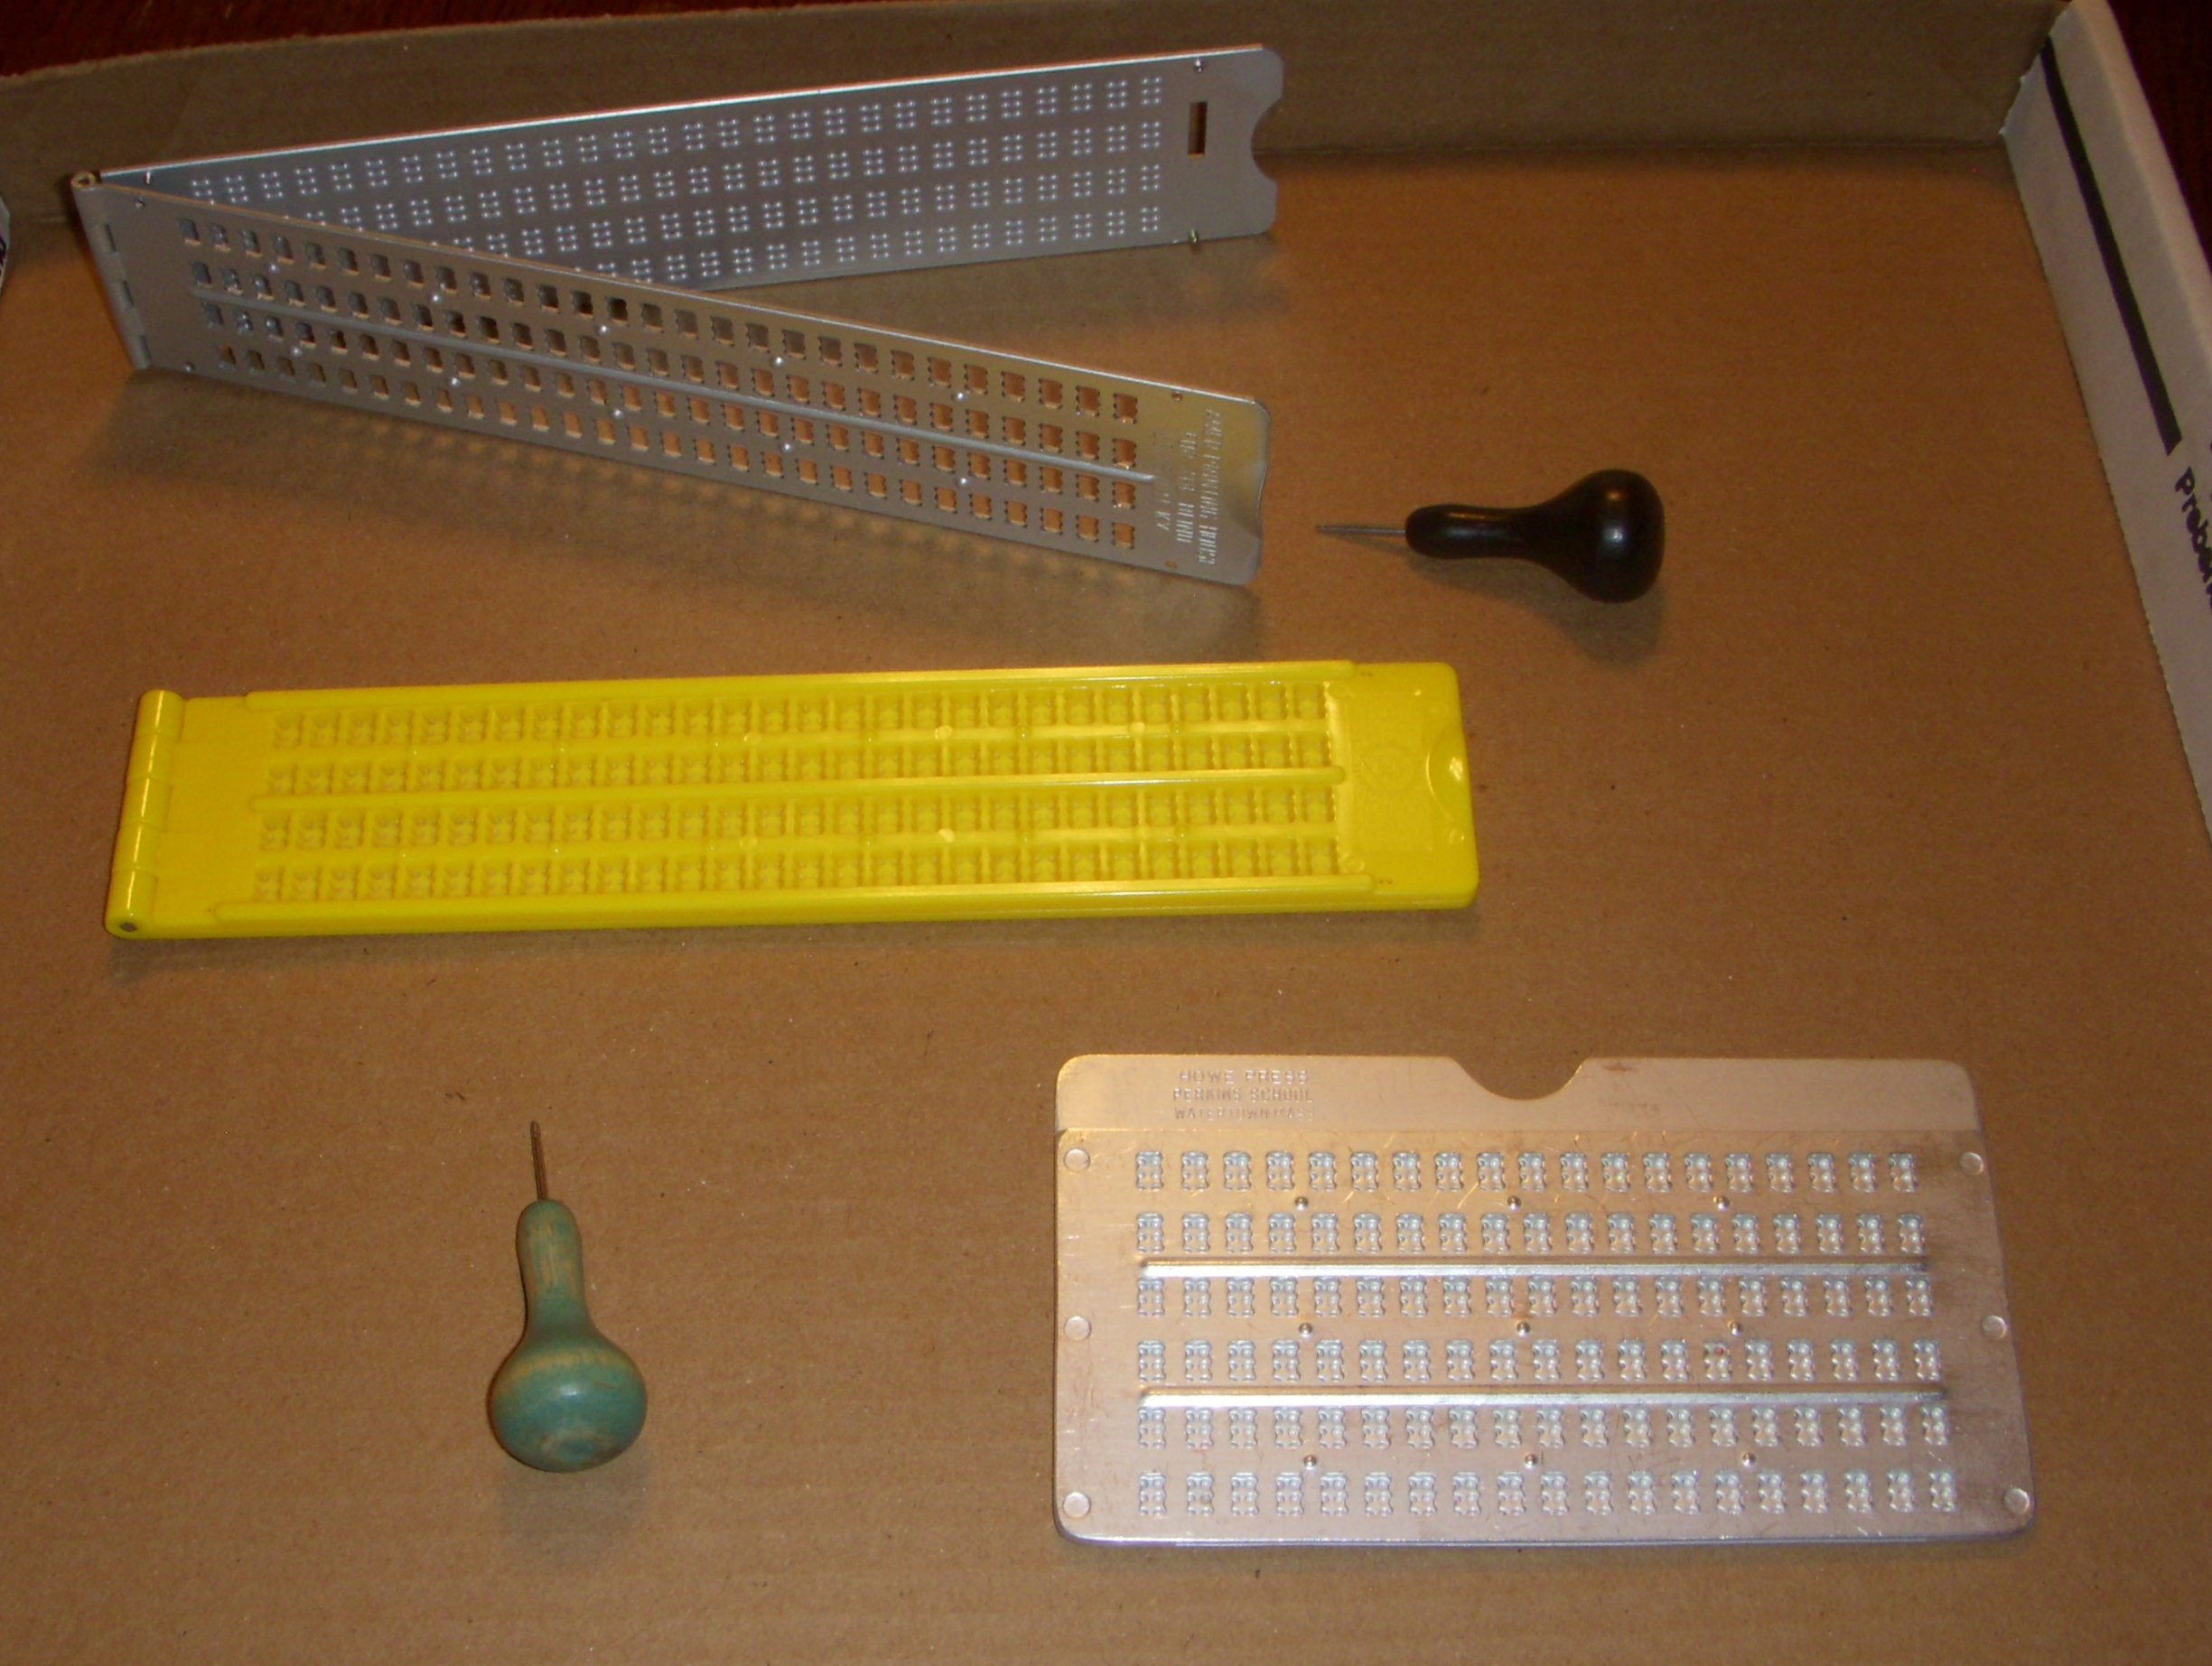
\includegraphics[width=12cm]{./img/Slate_and_Stylus_3.png}
\caption{Regletas y punzones para escritura braille.}
\label{fig:Slate_and_Stylus_3}
\end{figure}

Las principales desventajas de este m\'etodo, es que requiere que la persona
que escribe este muy capacitada y piense al revez\footnote{Esto se debe a que
en las regletas las celdas se escriben del lado opuesto a donde se leeran}
mientras lo hace, ademas de que se obtienen muy pocos caracteres por minuto.

\subsection{Maquina de escribir braille}
%
En 1892 Frank Haven Hall\footnote{V\'ease - \url{
http://books.google.com/books?id=u4uzPlgcWpsC&pg=PA452&lpg=PA452&dq=Frank+Haven
+Hall&source=bl&ots=Xf_e354ZC9&sig=2T51O8wSR92Vj1tWHBtySCBU0Bg&hl=es&ei=eClWSqy
AAcuwlAeC5ujcAg&sa=X&oi=book_result&ct=result&resnum=9}} invent\'o una maquina
compleja completamente mec\'anica pero de funcionamiento muy sencillo para la
escritura braille.\\

Hasta el dia de hoy las actuales maquinas de escribir braille se basan en los
mismos principios de funcionamientos que aquella que inven\'o Frank Haven Hall,
pero la teconolgia de fabricaci\'on se basa materiales m\'as livianos y
resistentes que los de aquella epoca. \\

El mecanismo consiste de una parte movil con movimientos horizontales donde se
fija el papel el cual puede a se vez desplazarse hacia arriba o hacia abajo
como en las maquinas de escribir comunes. Posee seis teclas que mueven un
juego de v\'astagos que a su vez activan una serie de punz\'ones que marcan la
hoja. Estas seis teclas permiten escribir (o impactar) un caracter braille a
la vez, y luego existe una s\'eptima tecla\footnote{Esto seria similar a la
barra espaciadora de las maquinas de escribir convencionales.} que se encaga de
desplazar la hoja hacia un lado permitiendo as\'i escribir un caracter nuevo.\\

Se puede ver en la figura \ref{fig:hallbraille-03} la maquina original
inventada por Frank Haven Hall, y en la figura
\ref{fig:ng_perkinsaph_brailler} se muestra un modelo nuevo que se puede
encontrar actualemten en el mercado.


% http://www.typewriter.be/hallbraille.htm
\begin{figure}[htp]
\centering
\includegraphics[width=10cm]{./img/hallbraille-03.png}
\caption{Primera maquina de escribir braille inventada por Frank Haven Hall
en 1892.}
\label{fig:hallbraille-03}
\end{figure}



%https://secure2.convio.net/psb/site/Ecommerce/1079514097?VIEW_PRODUCT=true&pro
%d uct_id=2041&store_id=1101
\begin{figure}[htp]
\centering
\includegraphics[width=10cm]{./img/ng_perkinsaph_brailler.png}
\caption{Maquina de escribir braille actual del mercado.}
\label{fig:ng_perkinsaph_brailler}
\end{figure}

Estas maquinas, al igual que la regleta y el punz\'on, requieren una persona
con conocimientos y pr\'actica para su uso, pero poseen la ventaja de que se
pueden lograr una mayor cantidad de caracteres por minuto. De hecho cuando
Frank Haven Hall present\'o su invento, impresion\'o a la audiencia con una
velocidad de 58 palabras por minuto.



\subsection{Impresoras braille}
%
La primera\footnote{V\'ease - \url{http://www.duxburysystems.com/bthist.asp}}
imresora braille\footnote{El t\'ermino correcto es \emph{impactadora} debido a
que proviene del ingl\'es \emph{embosser}} para papel normal fue fabricada en
el Instituto de Tecnologia de Masachusset (\emph{MIT - Massachusetts Institute
of Technology})\footnote{\url{http://web.mit.edu/}} a finales de la decada de
los 60 y se llam\'o \emph{BrailleEmboss} cuyo dise\~no estuvo a cargo de
George Dalrymple\footnote{\url{
http://www.ll.mit.edu/Retirees/Picnic05/index_04.html}}.\\
%% SEGUIR HABLANDO DE LA MISMA IMPRESORA %%%%



Existen actualmente en el mercado una amplia variedad de impresoras braille
para cubrir la mayoria de las necesidades de los usuarios, desde impresoras
personales hasta impresoras para grandes niveles de producci\'on.